\documentclass[tikz,border=2mm]{standalone}
\usepackage{amsmath}
\usepackage{amssymb}
\usepackage{tikz}
\usetikzlibrary{arrows.meta,positioning,fit,backgrounds,calc}

\definecolor{lightblue}{RGB}{173,216,230}
\definecolor{lightgreen}{RGB}{144,238,144}
\definecolor{lightyellow}{RGB}{255,250,205}
\definecolor{lightred}{RGB}{255,182,193}
\definecolor{edgegreen}{RGB}{42,135,58}
\definecolor{edgeorange}{RGB}{220,120,25}
\definecolor{edgepurple}{RGB}{135,55,150}

\begin{document}
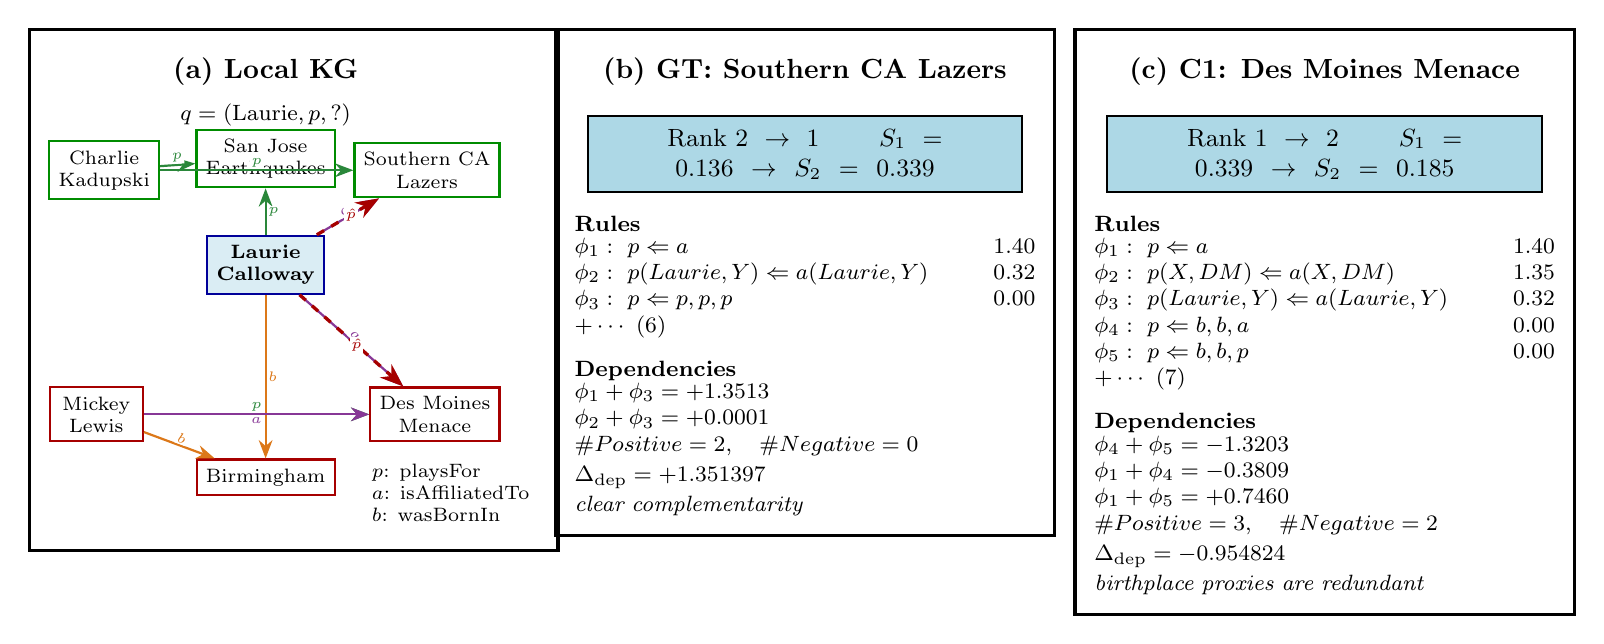
\begin{tikzpicture}[
    node distance=0.22cm,
    box/.style={rectangle, draw, thick, minimum width=2.8cm, minimum height=0.55cm, align=center, font=\small},
    title/.style={font=\bfseries\normalsize},
    formula/.style={font=\footnotesize, align=left},
    section/.style={rectangle, draw=black, very thick, inner sep=2.4mm},
    ent/.style={rectangle, draw, thick, minimum width=1.18cm, minimum height=0.42cm, align=center, font=\scriptsize},
    gt/.style={ent, fill=white, draw=green!55!black},
    c1/.style={ent, fill=white, draw=red!65!black},
    qent/.style={ent, fill=lightblue!45, draw=blue!60!black, font=\scriptsize\bfseries},
    plays/.style={-Stealth, thick, edgegreen},
    affil/.style={-Stealth, thick, edgepurple},
    born/.style={-Stealth, thick, edgeorange},
    pred/.style={-Stealth, very thick, dashed, red!65!black},
    elab/.style={font=\tiny, fill=white, inner sep=0.6pt},
    legend/.style={font=\scriptsize, align=left}
]

% ============ (a) Local KG ============
\node[title] (title-a) at (0,0) {(a) Local KG};
\node[formula] (query) at (0,-0.55) {$q=(\mathrm{Laurie},p,?)$};

\node[qent] (laurie) at (0.0,-2.45) {Laurie\\Calloway};
\node[gt] (scl) at (2.05,-1.25) {Southern CA\\Lazers};
\node[gt] (sje) at (0.0,-1.10) {San Jose\\Earthquakes};
\node[gt] (charlie) at (-2.05,-1.25) {Charlie\\Kadupski};
\node[c1] (dm) at (2.15,-4.35) {Des Moines\\Menace};
\node[c1] (birmingham) at (0.0,-5.15) {Birmingham};
\node[c1] (mickey) at (-2.15,-4.35) {Mickey\\Lewis};

\node[legend] (kg-legend) at (2.35,-5.35) {$p$: playsFor\\$a$: isAffiliatedTo\\$b$: wasBornIn};

\draw[affil] (laurie) -- node[elab,above,sloped] {$a$} (scl);
\draw[plays] (laurie) -- node[elab,right] {$p$} (sje);
\draw[plays] (charlie) -- node[elab,above,sloped] {$p$} (sje);
\draw[plays] (charlie) -- node[elab,above,sloped] {$p$} (scl);
\draw[affil] (laurie) -- node[elab,above,sloped] {$a$} (dm);
\draw[born] (laurie) -- node[elab,right] {$b$} (birmingham);
\draw[born] (mickey) -- node[elab,above,sloped] {$b$} (birmingham);
\draw[plays] (mickey) -- node[elab,above] {$p$} (dm);
\draw[affil] (mickey) -- node[elab,below,sloped] {$a$} (dm);
\draw[pred] (laurie) -- node[elab,pos=0.55] {$\hat p$} (scl);
\draw[pred] (laurie) -- node[elab,pos=0.55] {$\hat p$} (dm);

\begin{scope}[on background layer]
\node[section, fit=(title-a)(query)(laurie)(scl)(sje)(charlie)(dm)(birmingham)(mickey)(kg-legend)] (sec-a) {};
\end{scope}

% ============ (b) GT ============
\node[title] (title-b) at (6.85,0) {(b) GT: Southern CA Lazers};

\node[box, fill=lightblue, below=0.25cm of title-b, text width=5.2cm, inner sep=1.6mm] (gt-score) {
    Rank $2\to1$ \qquad
    $S_1=0.136 \to S_2=0.339$
};

\node[formula, below=0.28cm of gt-score, text width=5.85cm, inner sep=0mm] (gt-rules) {
    \textbf{Rules}\\[-0.5mm]
    $\phi_1:\ p\Leftarrow a$ \hfill $1.40$\\
    $\phi_2:\ p(Laurie,Y)\Leftarrow a(Laurie,Y)$ \hfill $0.32$\\
    $\phi_3:\ p\Leftarrow p,p,p$ \hfill $0.00$\\
    $+\cdots\ (6)$
};

\node[formula, below=0.28cm of gt-rules, text width=5.85cm, inner sep=0mm] (gt-dep) {
    \textbf{Dependencies}\\[-0.5mm]
    $\phi_1+\phi_3=+1.3513$\\
    $\phi_2+\phi_3=+0.0001$\\
    $\#Positive=2,\quad \#Negative=0$\\[0.5mm]
    $\Delta_{\rm dep}=+1.351397$\\[0.5mm]
    \textit{clear complementarity}
};

\begin{scope}[on background layer]
\node[section, fit=(title-b)(gt-score)(gt-rules)(gt-dep), inner sep=2.4mm] (sec-b) {};
\end{scope}

% ============ (c) C1 ============
\node[title] (title-c) at (13.45,0) {(c) C1: Des Moines Menace};

\node[box, fill=lightblue, below=0.25cm of title-c, text width=5.2cm, inner sep=1.6mm] (c1-score) {
    Rank $1\to2$ \qquad
    $S_1=0.339 \to S_2=0.185$
};

\node[formula, below=0.28cm of c1-score, text width=5.85cm, inner sep=0mm] (c1-rules) {
    \textbf{Rules}\\[-0.5mm]
    $\phi_1:\ p\Leftarrow a$ \hfill $1.40$\\
    $\phi_2:\ p(X,DM)\Leftarrow a(X,DM)$ \hfill $1.35$\\
    $\phi_3:\ p(Laurie,Y)\Leftarrow a(Laurie,Y)$ \hfill $0.32$\\
    $\phi_4:\ p\Leftarrow b,b,a$ \hfill $0.00$\\
    $\phi_5:\ p\Leftarrow b,b,p$ \hfill $0.00$\\
    $+\cdots\ (7)$
};

\node[formula, below=0.28cm of c1-rules, text width=5.85cm, inner sep=0mm] (c1-dep) {
    \textbf{Dependencies}\\[-0.5mm]
    $\phi_4+\phi_5=-1.3203$\\
    $\phi_1+\phi_4=-0.3809$\\
    $\phi_1+\phi_5=+0.7460$\\
    $\#Positive=3,\quad \#Negative=2$\\[0.5mm]
    $\Delta_{\rm dep}=-0.954824$\\[0.5mm]
    \textit{birthplace proxies are redundant}
};

\begin{scope}[on background layer]
\node[section, fit=(title-c)(c1-score)(c1-rules)(c1-dep), inner sep=2.4mm] (sec-c) {};
\end{scope}

\end{tikzpicture}
\end{document}
